% Created 2019-01-10 Thu 14:39
% Intended LaTeX compiler: pdflatex
\documentclass[11pt]{article}
\usepackage[utf8]{inputenc}
\usepackage[T1]{fontenc}
\usepackage{graphicx}
\usepackage{grffile}
\usepackage{longtable}
\usepackage{wrapfig}
\usepackage{rotating}
\usepackage[normalem]{ulem}
\usepackage{amsmath}
\usepackage{textcomp}
\usepackage{amssymb}
\usepackage{capt-of}
\usepackage{hyperref}
\input{/home/liam/main.tex}
\author{liam beckman}
\date{\today}
\title{Assignment 1}
\hypersetup{
 pdfauthor={liam beckman},
 pdftitle={Assignment 1},
 pdfkeywords={},
 pdfsubject={},
 pdfcreator={Emacs 26.1 (Org mode 9.1.9)}, 
 pdflang={English}}
\begin{document}

\maketitle
All information sourced from \href{https://wiki.dominionstrategy.com/}{wiki.dominionstrategy.com} under the Creative Commons Attribution Non-Commercial Share Alike License.

\noindent\rule{\textwidth}{0.5pt}

\section*{Smithy}
\label{sec:orgdc825c2}

\begin{center}
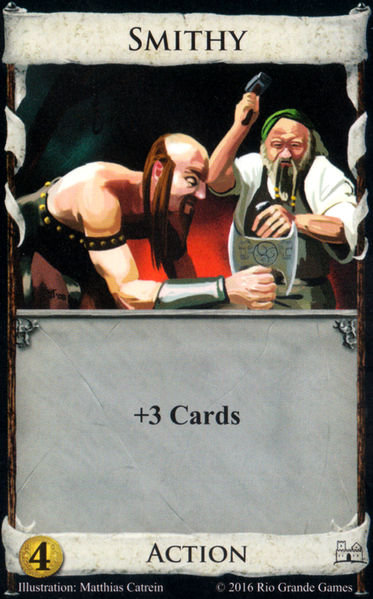
\includegraphics[width=0.25\linewidth]{./assets/smithy.jpg}
\end{center}

An action card with a cost of 4. When played, allows the player to draw an additional 3 cards into their hand.

\noindent\rule{\textwidth}{0.5pt}

\section*{Adventurer}
\label{sec:org50d9a35}

\begin{center}
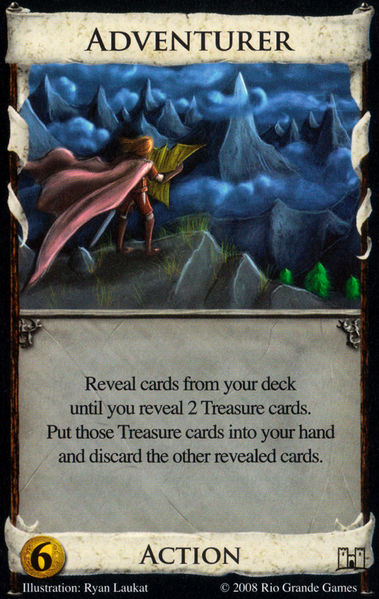
\includegraphics[width=0.25\linewidth]{./assets/adventurer.jpg}
\end{center}

An action card with a cost of 6. When played, the player must reveal cards from their deck until 2 treasure cards are found (e.g. Copper, Silver, Gold). The remanining revealed cards are then discarded.

\noindent\rule{\textwidth}{0.5pt}

\section*{Ambassador}
\label{sec:orgf48a349}


\begin{center}
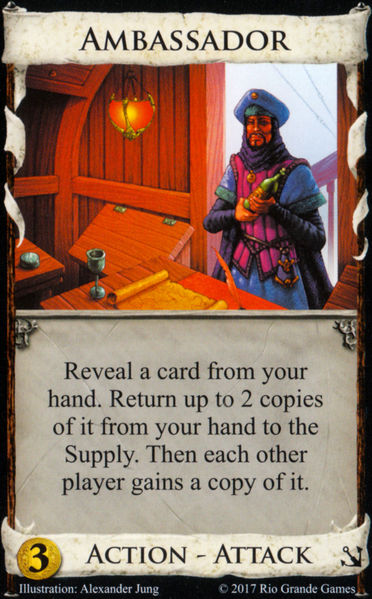
\includegraphics[width=0.25\linewidth]{./assets/ambassador.jpg}
\end{center}

An action-attack card with a cost of 3. Allows the player to transfer up to 2 copies of a particular card from their hand to their supply. Then each opponent receives 1 copy of that card.

\noindent\rule{\textwidth}{0.5pt}

\section*{Gardens}
\label{sec:org26d3738}


\begin{center}
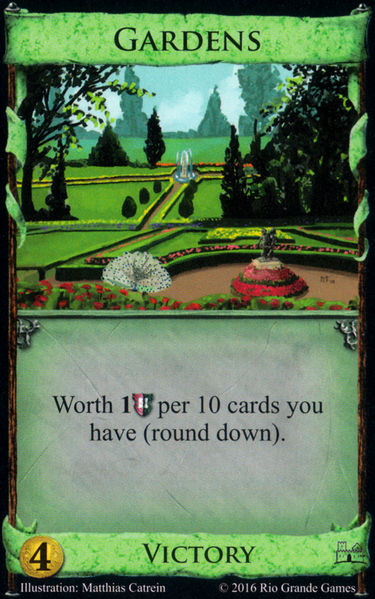
\includegraphics[width=0.25\linewidth]{./assets/gardens.jpg}
\end{center}

A victory card with a cost of 4. At the end of the round, it adds 1 victory point for every 10 cards in the player's hand.

\noindent\rule{\textwidth}{0.5pt}

\section*{Village}
\label{sec:org7af6c4e}


\begin{center}
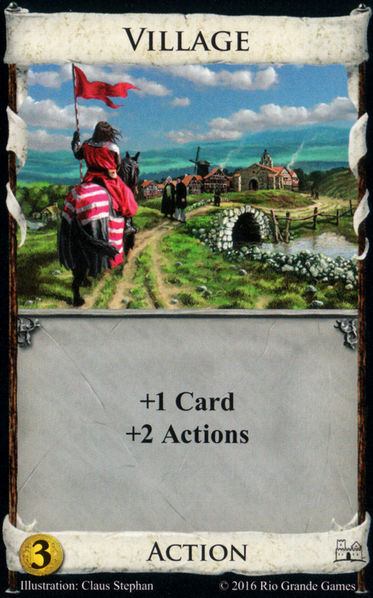
\includegraphics[width=0.25\linewidth]{./assets/village.jpg}
\end{center}

An action card with a cost of 3. Allows the player to draw 1 extra card from the deck, and play 2 additional actions.
\end{document}